\documentclass[11pt,a4paper]{article}

% ---------------------------------------------------------------------------
% Packages
% ---------------------------------------------------------------------------
\usepackage[margin=2.5cm]{geometry}
\usepackage[utf8]{inputenc}
\usepackage[T1]{fontenc}
\usepackage{graphicx}
\usepackage{tikz}
\usetikzlibrary{shapes.geometric, arrows.meta, positioning, fit, backgrounds, calc}
\usepackage{booktabs}
\usepackage{xcolor}
\usepackage{hyperref}
\usepackage{listings}
\usepackage{enumitem}
\usepackage{caption}
\usepackage{float}
\usepackage{parskip}
\usepackage{underscore}
\usepackage[export]{adjustbox}

\hypersetup{
    colorlinks=true,
    linkcolor=blue!50!black,
    citecolor=blue!50!black,
    urlcolor=blue!50!black,
    pdftitle={Phase 0 and Phase 1 Implementation Report},
    pdfauthor={Narges}
}

% ---------------------------------------------------------------------------
% Color palette for diagrams
% ---------------------------------------------------------------------------
\definecolor{dbcolor}{RGB}{215,235,250}
\definecolor{ontopcolor}{RGB}{255,235,205}
\definecolor{guicolor}{RGB}{225,245,225}
\definecolor{pipelinecolor}{RGB}{240,225,245}
\definecolor{regcolor}{RGB}{255,225,225}
\definecolor{boxborder}{RGB}{80,80,80}

\tikzset{
    block/.style={rectangle, draw=boxborder, rounded corners, thick,
        text width=3.1cm, minimum height=1.1cm, align=center, font=\small},
    smallblock/.style={rectangle, draw=boxborder, rounded corners, thick,
        text width=2.5cm, minimum height=0.9cm, align=center, font=\footnotesize},
    arrow/.style={-{Latex[length=2.5mm]}, thick}
}

% ---------------------------------------------------------------------------
% Listings style (used only for multi-line code/config blocks; all inline
% code in running text/captions uses \code{} instead, defined below, so
% that no fragile verbatim-like command ever appears inside a moving
% argument such as \caption{}).
% ---------------------------------------------------------------------------
\lstset{
    basicstyle=\ttfamily\footnotesize,
    breaklines=true,
    frame=single,
    backgroundcolor=\color{gray!7},
    columns=fullflexible,
    showstringspaces=false,
    xleftmargin=1em,
    xrightmargin=1em,
    aboveskip=8pt,
    belowskip=8pt
}

% \code{...}: robust inline monospace for identifiers/paths. Safe inside
% \caption{}, table cells, and tikz node text alike. Underscores must be
% written as \_ inside the argument.
\newcommand{\code}[1]{\texttt{#1}}

\title{\Large \textbf{A Multi-Domain Virtual Knowledge Graph Query System} \\[4pt]
\large Implementation Report --- Phase 0 (Data \& Infrastructure Preparation) \\
and Phase 1 (Domain-Switching Infrastructure) \\[2pt]
\normalsize \emph{Development \& evaluation harness for the query recommender}}
\author{Narges \\ \small Supervisor: Prof. Elisa Quintarelli}
\date{\today}

\begin{document}

\maketitle

\begin{abstract}
\noindent
This report documents the first two implementation phases of a thesis project centered on an
LLM-based query recommender for natural-language querying over Virtual Knowledge Graphs (VKGs).
\textbf{Phase 0} stands up two independent VKGs --- a synthetic \emph{Movie} domain and a real
\emph{Tourism} domain (Verona) --- each served through an Ontop OBDA endpoint over a
containerized PostgreSQL/PostGIS database. \textbf{Phase 1} adds a domain-switching mechanism on
top of the existing ``Indeewari'' NL2SPARQL pipeline so it can point at either VKG. Both phases
are complete and verified end-to-end. Following a scope decision made with the supervisor after
this work was completed (Section~\ref{sec:scope}), neither phase is a thesis deliverable in its
own right: they exist solely as an internal data/infrastructure \emph{harness} that the actual
contribution --- the query recommender, Phase 3 onward --- is developed and evaluated against.
Accordingly, this report focuses on the data and schema infrastructure the recommender depends on
(the two running VKGs, the domain registry, and a schema-format bug fix required to make the
Movie domain queryable at all) and omits implementation detail specific to the exploratory GUI
used only for local development, which is not part of the system's architecture going forward.
\end{abstract}

\tableofcontents
\newpage

% =============================================================================
\section{Introduction}
% =============================================================================

The base system, Indeewari, allows a non-expert user to type a natural-language question (e.g.\
\emph{``Churches in Verona''}) and receive results retrieved from a single, pre-wired Virtual
Knowledge Graph via an LLM-driven NL2SPARQL pipeline. The thesis extends this system along three
axes, in increasing order of research weight:

\begin{enumerate}[label=(\arabic*)]
    \item \textbf{Domain selection} --- generalize the application so a user can choose
        \emph{which} VKG to query (Movie vs.\ Tourism) instead of the system being wired to a
        single dataset.
    \item \textbf{User selection instead of login} --- let the user pick \emph{who they are}
        from a list of personas, so the system can reason about that user's preferences without
        implementing real authentication.
    \item \textbf{Query recommendation} --- the thesis's core contribution: after answering a
        query, propose three follow-up query suggestions, conditioned on both the user's stated
        queries \emph{and} their real interaction behavior.
    \end{enumerate}

This report covers the two phases completed so far: \textbf{Phase 0}, which prepares the data
and infrastructure needed by every later phase, and \textbf{Phase 1}, which delivers item (1)
above. Phases 2--6 (user selection, behavioral profiling, the recommender core, evaluation, and
thesis writing) are documented separately in the project roadmap and are out of scope here.

\subsection{Scope narrowing (post-implementation)}
\label{sec:scope}

After Phases 0 and 1 were implemented and verified, an email exchange with the supervisor
narrowed the thesis scope: items (1) domain selection and (2) user selection instead of login are
\textbf{not thesis deliverables} --- they are owned by a separate application already built by
two bachelor students under the same supervisor. The thesis's entire contribution is item (3),
the query recommender, delivered as a \textbf{standalone model and API} that any caller
(including the bachelor students' application) can integrate independently. This report is
written after that decision and reflects it: the two VKGs and domain-registry infrastructure
described below are retained only as an \textbf{internal development and evaluation harness} ---
a way to build and demo the recommender against real schemas and data without depending on the
external application's timeline or codebase. The exploratory Streamlit GUI that was built during
Phase 1 to exercise this harness manually is not described here in implementation detail, since
it is disposable dev tooling rather than part of the system's architecture; what matters going
forward is that both VKGs are live, queryable, and switchable in configuration, which is what the
rest of this report documents.

% =============================================================================
\section{High-Level System Overview}
% =============================================================================

\subsection{Overview}

Before Phase 0/1, the NL2SPARQL pipeline queried a single, hardcoded SPARQL endpoint with no
notion of alternate domains. After these two phases, the system consists of two layers stacked
on top of the unchanged pipeline core: a containerized \textbf{data/infrastructure layer}
(Docker Compose services running Postgres, PostGIS, and two Ontop VKG endpoints), and a
\textbf{registry layer} (a YAML file listing which knowledge graphs are available, plus a small
Python loader). A thin, dev-only harness consumes the registry to point the pipeline's
in-memory configuration (SPARQL endpoint URL, schema path) at whichever domain is being tested;
per Section~\ref{sec:scope}, this harness is not part of the system's architecture going
forward, so it is omitted from the diagram below. Figure~\ref{fig:high-level} shows how the two
retained layers connect to the pipeline.

\begin{figure}[H]
\centering
\begin{adjustbox}{max width=\textwidth, max totalheight=0.85\textheight, center}
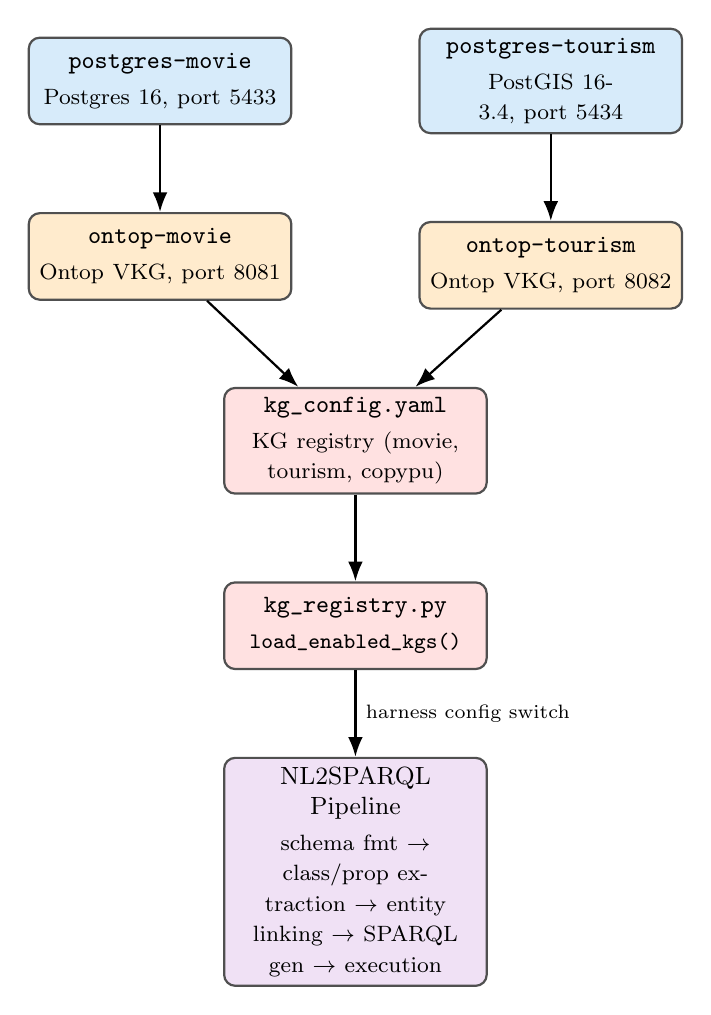
\begin{tikzpicture}[node distance=1.1cm and 1.3cm]

    % Layer 1: Docker infrastructure
    \node[block, fill=dbcolor] (pgm) {\code{postgres-movie}\\[2pt]\footnotesize Postgres 16, port 5433};
    \node[block, fill=dbcolor, right=1.6cm of pgm] (pgt) {\code{postgres-tourism}\\[2pt]\footnotesize PostGIS 16-3.4, port 5434};

    \node[block, fill=ontopcolor, below=of pgm] (om) {\code{ontop-movie}\\[2pt]\footnotesize Ontop VKG, port 8081};
    \node[block, fill=ontopcolor, below=of pgt] (ot) {\code{ontop-tourism}\\[2pt]\footnotesize Ontop VKG, port 8082};

    % Layer 2: Registry
    \coordinate (midOmOt) at ($(om)!0.5!(ot)$);
    \node[block, fill=regcolor, below=1.6cm of midOmOt] (reg) {\code{kg\_config.yaml}\\[2pt]\footnotesize KG registry (movie, tourism, copypu)};

    \node[block, fill=regcolor, below=of reg] (regpy) {\code{kg\_registry.py}\\[2pt]\footnotesize \code{load\_enabled\_kgs()}};

    % Layer 3: Pipeline
    \node[block, fill=pipelinecolor, below=of regpy] (pipe) {NL2SPARQL Pipeline\\[2pt]\footnotesize schema fmt $\to$ class/prop extraction $\to$ entity linking $\to$ SPARQL gen $\to$ execution};

    \draw[arrow] (pgm) -- (om);
    \draw[arrow] (pgt) -- (ot);
    \draw[arrow] (om) -- (reg);
    \draw[arrow] (ot) -- (reg);
    \draw[arrow] (reg) -- (regpy);
    \draw[arrow] (regpy) -- node[right,font=\scriptsize]{harness config switch} (pipe);

\end{tikzpicture}
\end{adjustbox}
\caption{High-level architecture after Phase 0/1: containerized VKGs (bottom-up: database
$\to$ Ontop endpoint) feed a configuration registry, which a thin dev-only harness (not shown,
Section~\ref{sec:scope}) reads to reconfigure the unmodified NL2SPARQL pipeline at runtime.}
\label{fig:high-level}
\end{figure}

\subsection{In depth: what changed and what did not}

The NL2SPARQL pipeline itself --- schema formatting, class/property relevance extraction, entity
linking, SPARQL generation, execution, and result formatting --- is \textbf{unmodified}. Both
phases only add infrastructure and configuration \emph{around} it:

\begin{itemize}
    \item Phase 0 adds two new SPARQL endpoints the pipeline can point at, each backed by a real
        relational database exposed as RDF through an Ontop OBDA mapping.
    \item Phase 1 adds a way to \emph{choose} which endpoint (and which corresponding schema
        file) the pipeline uses for a given session, replacing what used to be a single
        hardcoded configuration.
    \end{itemize}

This design choice keeps the two completed phases low-risk: because the pipeline's internals are
untouched, any bug introduced by these phases is necessarily located in the new infrastructure or
the new selector code, not in query answering logic that was already tested.

\newpage
% =============================================================================
\section{Phase 0 --- Data \& Infrastructure Preparation}
% =============================================================================

\subsection{Overview}

Phase 0's goal is to give the system two real, queryable Virtual Knowledge Graphs to switch
between in Phase 1: a \textbf{Movie} domain (synthetic Netflix-shaped dataset, chosen so it can
later carry per-user behavioral signals for the thesis's recommender) and a \textbf{Tourism}
domain (a real 293\,MB production database dump of Verona's tourism application, inherited from
the Indeewari predecessor project). Each domain is stood up as an isolated Docker Compose stack:
a relational database container feeding an Ontop container that exposes the data as a VKG over
SPARQL. Figure~\ref{fig:phase0} shows the four services and their dependencies.

\begin{figure}[H]
\centering
\begin{adjustbox}{max width=0.85\textwidth, max totalheight=0.7\textheight, center}
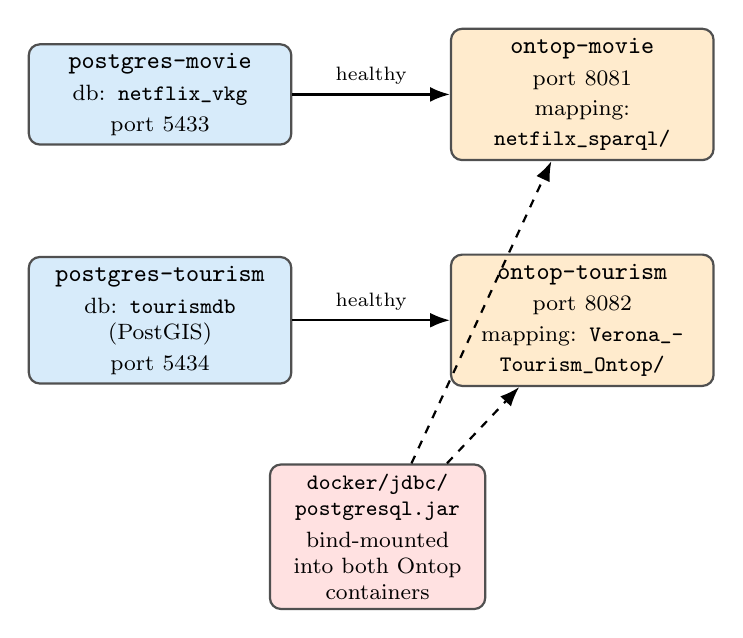
\begin{tikzpicture}[node distance=1.4cm and 2cm]

    \node[block, fill=dbcolor] (pgm) {\code{postgres-movie}\\[2pt]\footnotesize db: \code{netflix\_vkg}\\ port 5433};
    \node[block, fill=ontopcolor, right=of pgm] (om) {\code{ontop-movie}\\[2pt]\footnotesize port 8081\\ mapping: \code{netfilx\_sparql/}};

    \node[block, fill=dbcolor, below=of pgm] (pgt) {\code{postgres-tourism}\\[2pt]\footnotesize db: \code{tourismdb} (PostGIS)\\ port 5434};
    \node[block, fill=ontopcolor, right=of pgt] (ot) {\code{ontop-tourism}\\[2pt]\footnotesize port 8082\\ mapping: \code{Verona\_Tourism\_Ontop/}};

    \node[smallblock, fill=regcolor, below right=1.0cm and -0.3cm of pgt] (jdbc) {\code{docker\slash{}jdbc\slash{}postgresql.jar}\\[2pt]\footnotesize bind-mounted into both Ontop containers};

    \draw[arrow] (pgm) -- node[above,font=\scriptsize]{healthy} (om);
    \draw[arrow] (pgt) -- node[above,font=\scriptsize]{healthy} (ot);
    \draw[arrow, dashed] (jdbc) -- (om);
    \draw[arrow, dashed] (jdbc) -- (ot);

\end{tikzpicture}
\end{adjustbox}
\caption{Docker Compose topology for Phase 0. Each Ontop container waits for its database's
healthcheck (\code{depends\_on: service\_healthy}) before starting, and both mount the same JDBC
driver directory (dashed arrows) to work around a missing-driver issue in the base Ontop image
(Section~\ref{sec:bugs}).}
\label{fig:phase0}
\end{figure}

\subsection{Movie domain VKG}

The Movie side uses the richer of two available Movie datasets in the repository ---
\code{netfilx\_sparql/} (ontology + OBDA mapping) combined with \code{netflix\_dataset/} (the
actual CSV data) --- rather than a smaller, cleaner but behaviorally-empty alternative
(\code{Movie/}) that has no user, search, or watch-history concept and therefore cannot support
the thesis's later behavioral-profiling work.

\code{postgres-movie} is initialized from \code{docker/movie/init.sql}, which creates six tables
loaded from the \code{netflix\_dataset/} CSVs:

\begin{table}[H]
\centering
\begin{tabular}{lrl}
\toprule
\textbf{Table} & \textbf{Rows} & \textbf{Role} \\
\midrule
\code{movies}              & 1{,}040   & Catalog \\
\code{users}               & 10{,}300  & User master data \\
\code{watch\_history}       & 105{,}000 & Real behavior (implicit feedback) \\
\code{search\_logs}         & 26{,}500  & Stated intent (free-text search) \\
\code{reviews}             & 15{,}450  & Explicit stated opinions \\
\code{recommendation\_logs} & 52{,}000  & System-suggested vs.\ consumed \\
\bottomrule
\end{tabular}
\caption{Movie domain tables in \code{postgres-movie}, with row counts verified against the
source CSVs exactly.}
\label{tab:movie-tables}
\end{table}

\noindent A deliberate design choice: \textbf{no table has a primary key}. The source dataset
contains genuine duplicate id values across every table (e.g.\ roughly 40 of the 1{,}040
\code{movie\_id} values repeat), so plain non-unique indexes are used instead of primary keys,
and the init script's comments record this decision explicitly so it is not mistaken for an
oversight later.

Two categories of fixes were required to the pre-existing ontology and OBDA mapping under
\code{netfilx\_sparql/}:

\begin{itemize}
    \item \textbf{Bug fix}: the \code{watch-details} mapping in \code{netflix\_ontology.obda}
        originally selected a column named \code{watch\_duration}, which does not exist --- the
        real column is \code{watch\_duration\_minutes}. The mapping was corrected accordingly.
    \item \textbf{Coverage extension}: the mapping set was extended from its original scope to
        \textbf{17 mappings in total}, adding the columns needed by a later phase's
        search-to-watch temporal join: \code{search-details} (\code{searchDate}),
        \code{watch-session-details} (\code{watchDate}, \code{action}, \code{deviceType}),
        \code{recommendation-date} (\code{recommendationDate}), and a new object-property
        mapping, \code{watch-session-user}, connecting \code{WatchSession} to \code{User} via a
        new \code{watchedByUser} property (this relationship did not exist before, despite
        \code{WatchSession $\to$ Movie} and \code{WatchSession $\to$ Device} already being
        present). \code{netflix\_ontology.owl} was updated in lockstep with each new property,
        annotated with an explanatory comment marking it as an addition.
\end{itemize}

\begin{lstlisting}[language=SQL, caption={Excerpt of docker/movie/init.sql: the watch\_history
table, whose column naming mismatch with the original OBDA mapping was one of the bugs fixed in
this phase.}]
CREATE TABLE watch_history (
    session_id                 TEXT,
    user_id                    TEXT,
    movie_id                   TEXT,
    action                     TEXT,     -- started / paused / stopped / completed
    progress_percentage        NUMERIC,
    watch_duration_minutes     INTEGER,  -- NOTE: not "watch_duration"
    watch_date                 DATE,
    device_type                TEXT,
    user_rating                NUMERIC
    -- no PRIMARY KEY: source data has duplicate ids, see script header comment
);
\end{lstlisting}

\subsection{Tourism domain VKG}
\label{sec:tourism-vkg}

The Tourism side reuses \code{Verona\_Tourism\_Ontop/}, which contains a real production
PostgreSQL dump (\code{tourismdb\_jan 1.backup}, 293\,MB) of Verona's tourism application,
together with an ontology (\code{art\_all.ttl}) that --- unlike either Movie option --- already
embeds SHACL node shapes per class, a direct structural match for the pipeline's schema loader
(see Section~\ref{sec:shacl-fix}).

\code{postgres-tourism} runs on the PostGIS-enabled image (\code{postgis/postgis:16-3.4}),
because the source database uses \code{geometry}\slash\code{geography} columns that a plain Postgres
image cannot represent. It is initialized by \code{docker/tourism/restore.sh}, which first
creates the \code{postgis} extension and then restores the backup via
\code{pg\_restore --no-owner --jobs=2}, tolerating \code{pg\_restore}'s common non-fatal warning
exit codes rather than treating them as failures.

\begin{table}[H]
\centering
\begin{tabular}{lr}
\toprule
\textbf{Table} & \textbf{Rows} \\
\midrule
\code{art}      & 41 \\
\code{event}    & 1{,}416 \\
\code{calendar} & 10{,}640 \\
\code{location} & 1{,}600 \\
\bottomrule
\end{tabular}
\caption{Tourism domain tables in \code{postgres-tourism}, row counts verified against the
source backup exactly.}
\label{tab:tourism-tables}
\end{table}

The original OBDA mapping (\code{art\_all.obda}) shipped with 2 broken mappings,
\code{art-image-mapping} and \code{art-to-image-mapping}, which reference a table
\code{art\_images(art\_id, image\_url, caption, image\_type)} that does not exist anywhere in the
backup (only a differently-shaped legacy \code{oldapp.art\_media} table exists). Rather than
reconstructing the missing table, \textbf{these two mappings were dropped entirely} --- a
decision made explicitly with the professor's/user's sign-off, since art images are not needed
for the thesis demo. 14 mappings remain functional:

\begin{quote}\footnotesize\raggedright
\code{status-mapping}, \code{art-mapping}, \code{art-category-mapping},
\code{art-category-art-mapping}, \code{tour-type-mapping}, \code{tour-mapping},
\code{tour-art-mapping}, \code{event-mapping}, \code{event-category-mapping},
\code{event-category-event-mapping}, \code{calendar-mapping}, \code{location-mapping},
\code{event-to-location-mapping}, \code{event-to-calendar-mapping}.
\end{quote}

The classes/properties \code{ex:ArtImage}, \code{ex:hasImage}, and \code{ex:imageOfArt} remain
declared in \code{art\_all.ttl} for documentation purposes but are now unpopulated and unused.

\paragraph{Explicit scope decision.}
\label{par:tourism-scope}
The backup also contains a large behavioral table,
\code{log\_vc} (4.4 million rows of VeronaCard tap-in visits), which could in principle serve as
a behavioral signal analogous to the Movie domain's \code{watch\_history}. However,
\code{log\_vc} identifies an anonymous card, not a named person, and the database's only
\code{User}-like table (\code{auth\_user}) has just 4 admin/staff rows, not tourists.
\textbf{It was decided with the user that Tourism stays catalog-query-only for this thesis}:
\code{log\_vc} is not mapped into the ontology, and all user-selection/behavior-aware work in
later phases is carried entirely by the Movie domain. This is recorded here as a load-bearing
scope decision, not an oversight, since it bounds what later phases can demonstrate on the
Tourism side.

\subsection{Bugs discovered during bring-up}
\label{sec:bugs}

Two problems surfaced only once the containers were actually started, and were not anticipated
by the original infrastructure design:

\begin{enumerate}
    \item \textbf{Missing JDBC driver.} The base \code{ontop/ontop} Docker image ships with no
        JDBC drivers under \code{/opt/ontop/jdbc/}. Both Ontop containers failed at startup with
        \code{Cannot load the driver: org.postgresql.Driver}. \textbf{Fix}: the PostgreSQL JDBC
        driver (version 42.7.4) was downloaded into a new, gitignored directory,
        \code{docker/jdbc/}, and bind-mounted into both \code{ontop-*} services at
        \code{/opt/ontop/jdbc} in \code{docker-compose.yml}.
    \item \textbf{Comment syntax rejected by the OBDA parser.} Ontop's native \code{.obda} file
        parser rejects free-standing \code{\#} comment lines anywhere in the file, not only
        inside the mapping block. An explanatory comment describing the two dropped art-image
        mappings had to be removed from \code{art\_all.obda}; the same explanation is preserved
        in this report (Section~\ref{sec:tourism-vkg} above) and in the operational
        \code{docker/README.md} instead.
\end{enumerate}

\subsection{Credential hygiene}

Two legacy Ontop \code{.properties} files (\code{netfilx\_sparql\slash{}netflix\_ontology.properties}
and \code{Movie\slash{}movie\_project.properties}) originally contained plaintext database passwords.
Both now carry a \code{jdbc.password=CHANGEME} placeholder with an explanatory comment ---
neither file is actually read by the Docker Compose stack, which instead sources real
credentials from a gitignored root \code{.env} file (\code{POSTGRES\_MOVIE\_PASSWORD},
\code{POSTGRES\_TOURISM\_PASSWORD}), templated in a committed \code{.env.example}.

\subsection{Verification}

Phase 0 was verified in two ways:

\begin{itemize}
    \item \textbf{Row-count checks}: every table in Tables~\ref{tab:movie-tables} and
        \ref{tab:tourism-tables} was confirmed to match its source CSV/backup exactly.
    \item \textbf{SPARQL smoke tests}: two manual queries, documented with exact \code{curl}
        commands in \code{docker/README.md} --- a movie-title query against
        \code{:8081/sparql}, and an \code{ArtCategory} query against \code{:8082/sparql} that
        returns all six category names, including \textbf{``Chiese''} (churches), directly
        matching the professor's own example question, ``Churches in Verona.''
\end{itemize}

\newpage
% =============================================================================
\section{Phase 1 --- Domain-Switching Infrastructure}
% =============================================================================

\subsection{Overview}

Phase 1's goal is to let the NL2SPARQL pipeline be pointed, at runtime, at either VKG (Movie or
Tourism) or the pre-existing \code{copypu} maritime dataset, replacing what was previously a
single hardcoded SPARQL endpoint. As established in Section~\ref{sec:scope}, domain selection
itself is not a thesis deliverable --- it is the responsibility of the bachelor students'
external application --- so this section documents only the two pieces of infrastructure that
the recommender harness genuinely depends on: a declarative \textbf{KG registry} that any caller
can read to discover available domains and their endpoints, and a schema-format fix that was
required before the Movie domain's schema could be consumed at all. (A minimal Streamlit control
was used locally during development to exercise this registry by hand; its implementation is not
documented here, per Section~\ref{sec:scope}.) Figure~\ref{fig:phase1} traces how a domain is
resolved from the registry to a schema the pipeline can use.

\begin{figure}[H]
\centering
\begin{adjustbox}{max width=0.8\textwidth, max totalheight=0.6\textheight, center}
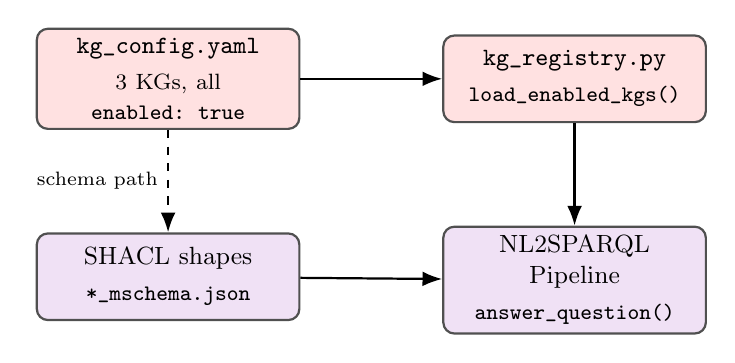
\begin{tikzpicture}[node distance=1.3cm and 1.8cm]

    \node[block, fill=regcolor] (yaml) {\code{kg\_config.yaml}\\[2pt]\footnotesize 3 KGs, all \code{enabled: true}};
    \node[block, fill=regcolor, right=of yaml] (regpy) {\code{kg\_registry.py}\\[2pt]\footnotesize \code{load\_enabled\_kgs()}};

    \node[block, fill=pipelinecolor, below=of yaml] (shacl) {SHACL shapes\\[2pt]\footnotesize \code{*\_mschema.json}};
    \node[block, fill=pipelinecolor, below=of regpy] (pipe) {NL2SPARQL Pipeline\\[2pt]\footnotesize \code{answer\_question()}};

    \draw[arrow] (yaml) -- (regpy);
    \draw[arrow] (regpy) -- (pipe);
    \draw[arrow] (shacl) -- (pipe);
    \draw[arrow, dashed] (yaml) -- node[left,font=\scriptsize]{schema path} (shacl);

\end{tikzpicture}
\end{adjustbox}
\caption{Phase 1 domain resolution: a caller (harness or, eventually, the recommender API) reads
the registry to obtain a domain's endpoint and schema path. The dashed edge denotes that the
schema referenced by the registry must already exist as valid SHACL --- the gap addressed in
Section~\ref{sec:shacl-fix} for the Movie domain.}
\label{fig:phase1}
\end{figure}

\subsection{The KG registry}

\code{web\_app/config/kg\_config.yaml} lists the available knowledge graphs. Each entry carries a
name, a schema file path, a SPARQL endpoint URL, a \code{source\_type}, and an \code{enabled}
flag:

\begin{table}[H]
\centering
\begin{tabular}{lll l}
\toprule
\textbf{Name} & \textbf{Schema file} & \textbf{Endpoint} & \textbf{source\_type} \\
\midrule
\code{copypu}   & \code{data/input/copypu.ttl}            & \code{:8080/sparql} & \code{local\_rdf} \\
\code{movie}    & \code{netfilx\_sparql/netflix\_ontology.owl} & \code{:8081/sparql} & \code{sparql\_endpoint} \\
\code{tourism}  & \code{Verona\_Tourism\_Ontop/art\_all.ttl}  & \code{:8082/sparql} & \code{sparql\_endpoint} \\
\bottomrule
\end{tabular}
\caption{The three enabled entries in kg\_config.yaml (a fourth, dbpedia, exists commented-out
and disabled).}
\label{tab:kg-registry}
\end{table}

This file previously existed as a documentation-only registry with no code reading it. Phase 1
introduces the first consumer, \code{web\_app/nl2sparql/kg\_registry.py}, whose
\code{load\_enabled\_kgs()} function parses the YAML and returns the entries whose
\code{enabled} flag is true, in file order (an empty list if the file is missing).

\subsection{The SHACL gap and its fix (Movie domain)}
\label{sec:shacl-fix}

The pipeline's only schema loader, \code{SHACLSchemaParser.parse()}
(\code{nl2sparql/schema\_parser.py}), builds the schema entirely from SHACL \code{sh:NodeShape}
triples --- it has \textbf{no fallback} that reads plain \code{rdfs:domain}\slash\code{rdfs:range}
declarations. The Movie ontology (\code{netflix\_ontology.owl}) is a plain RDF/XML OWL file with
zero SHACL triples, so feeding it directly to the parser silently produced an \textbf{empty
schema} --- the Movie domain would have appeared selectable in the GUI but answered every
question incorrectly.

\begin{figure}[H]
\centering
\begin{adjustbox}{max width=0.85\textwidth, max totalheight=0.6\textheight, center}
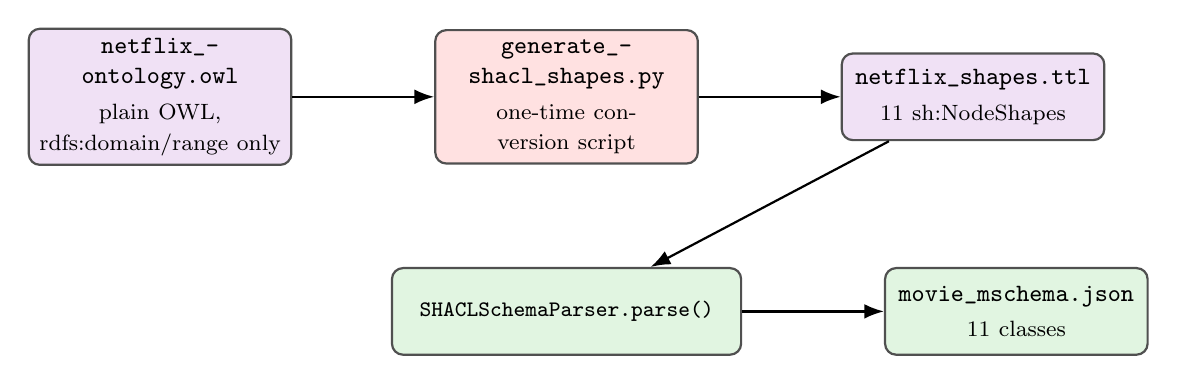
\begin{tikzpicture}[node distance=1.3cm and 1.8cm]
    \node[block, fill=pipelinecolor] (owl) {\code{netflix\_ontology.owl}\\[2pt]\footnotesize plain OWL, rdfs:domain/range only};
    \node[block, fill=regcolor, right=of owl] (script) {\code{generate\_shacl\_shapes.py}\\[2pt]\footnotesize one-time conversion script};
    \node[block, fill=pipelinecolor, right=of script] (shapes) {\code{netflix\_shapes.ttl}\\[2pt]\footnotesize 11 sh:NodeShapes};
    \node[block, fill=guicolor, below=of script, text width=4.2cm, font=\footnotesize] (parser) {\code{SHACLSchemaParser.parse()}};
    \node[block, fill=guicolor, right=of parser] (mschema) {\code{movie\_mschema.json}\\[2pt]\footnotesize 11 classes};

    \draw[arrow] (owl) -- (script);
    \draw[arrow] (script) -- (shapes);
    \draw[arrow] (shapes) -- (parser);
    \draw[arrow] (parser) -- (mschema);
\end{tikzpicture}
\end{adjustbox}
\caption{The Movie ontology has no SHACL shapes, so a one-time script generates them from its
existing rdfs:domain/range declarations before the pipeline's schema parser can consume it. The
Tourism ontology needed no such step, since art\_all.ttl already embeds SHACL shapes directly.}
\label{fig:shacl-fix}
\end{figure}

The fix is a new one-time script, \code{netfilx\_sparql\slash{}generate\_shacl\_shapes.py}: for every
\code{owl:Class} it emits an \code{sh:NodeShape} and \code{sh:targetClass}; for every property
whose \code{rdfs:domain} matches that class, it emits an \code{sh:property} blank node, using
\code{sh:class} + \code{sh:nodeKind sh:IRI} for object properties, or \code{sh:datatype} for
datatype properties. The output, \code{netfilx\_sparql\slash{}netflix\_shapes.ttl}, contains 11 node
shapes --- one per class (\code{Country}, \code{Device}, \code{Genre}, \code{Language},
\code{Movie}, \code{Recommendation}, \code{Review}, \code{Search}, \code{SubscriptionPlan},
\code{User}, \code{WatchSession}).

\subsection{Generated m-schema artifacts}

Both domains' machine-readable schema representations (the ``m-schema'' JSON format the
pipeline's later stages consume) were generated via \code{pipeline.extract\_schema()} and
committed under \code{web\_app/data/output/}:

\begin{itemize}
    \item \code{movie\_mschema.json} --- 11 classes, matching the 11 generated node shapes. Four
        classes (\code{Country}, \code{Device}, \code{Genre}, \code{Language},
        \code{SubscriptionPlan}) carry only a class label with no properties, since nothing else
        in the ontology targets them as an object-property range.
    \item \code{tourism\_mschema.json} --- 7 classes (e.g.\ \code{example:Art},
        \code{example:ArtCategory}), generated directly from the already-SHACL-shaped
        \code{art\_all.ttl} with no intermediate conversion step required.
\end{itemize}

\subsection{Verification}

Phase 1 was verified along two lines, both without requiring an LLM API key (no key was
configured in the verification environment, so only the non-LLM stages of the pipeline were
exercised directly):

\begin{enumerate}
    \item \textbf{Endpoint correctness}: direct SPARQL queries against both live Ontop endpoints
        confirmed the generated shapes' property IRIs match real data --- e.g.\ \code{ex:title}
        on \code{ex:Movie} returns real titles, and the Tourism \code{ArtCategory} query still
        returns ``Chiese.''
    \item \textbf{Schema-stage correctness}: running the pipeline's embedding-based class/property
        extraction stage against both new schemas correctly identified \code{Movie}\slash\code{Genre}
        + \code{hasGenre}\slash\code{title}\slash\code{releaseYear} for \emph{``What movies have the genre
        Action?''}, and \code{Art}\slash\code{ArtCategory}\slash\code{Event} + \code{artname\_it}/etc.\ for
        \emph{``Churches in Verona.''}
\end{enumerate}

\noindent Verification of the dev-only Streamlit control used to exercise this registry by hand
(domain-switch logic, browser reachability) is not reported here, consistent with
Section~\ref{sec:scope} excluding that tooling from the system's documented architecture.

\newpage
% =============================================================================
\section{Known Limitations and Open Items}
% =============================================================================

\begin{itemize}
    \item \textbf{Tourism has no per-user behavioral signal}, by explicit design decision rather
        than oversight (see the Tourism scope decision, Section~\ref{par:tourism-scope}): this bounds what later
        phases (user selection, behavior-aware recommendation) can demonstrate on the Tourism
        side --- that work is carried entirely by the Movie domain.
    \item \textbf{Neither Phase 0 nor Phase 1 is a thesis deliverable} as of the scope decision in
        Section~\ref{sec:scope}. Both are retained solely as the data/infrastructure harness that
        Phase 3 onward (the recommender) is built and evaluated against.
    \item \code{kg\_config.yaml} is currently consumed only by the dev-only harness described in
        Section~\ref{sec:scope}; no other part of \code{web\_app}, and no part of the recommender
        API itself, reads it yet. The eventual API contract for domain selection (if any) is an
        open question tracked in the project roadmap, not resolved by this report.
\end{itemize}

% =============================================================================
\section{Summary and Next Steps}
% =============================================================================

Phases 0 and 1 deliver a working, verified foundation: two real VKGs running behind Ontop,
switchable via a declarative registry, without touching the NL2SPARQL pipeline's core logic. Per
the scope decision in Section~\ref{sec:scope}, this foundation is now purely a development
harness; the thesis's actual contribution builds on top of it:

\begin{itemize}
    \item \textbf{Phase 3} (complete, documented separately in \emph{Phase 3 Implementation
        Report}) --- a behavioral preference profile extending the Movie domain's
        \code{watch\_history}\slash\code{search\_logs} data into a ``stated vs.\ actual preference''
        signal, the empirical basis for the thesis's core contribution.
    \item \textbf{Phase 4} --- the query recommender itself: LLM-based candidate generation
        grounded in both query history and the Phase 3 behavioral signal, with schema-validation
        and ranking before three suggestions are shown to the user, delivered as a standalone API.
    \item \textbf{Phases 5--6} --- evaluation and thesis writing.
\end{itemize}

\noindent Full detail on these phases is tracked in the project roadmap document,
\emph{Thesis Project Plan}, which also documents the four literature references (ADBIS 2026,
GQR/RA-GQR, the LLM+KG roadmap survey, and QRMOCCGA) that ground the recommender's design.

\end{document}
